\documentclass[10pt]{beamer}
% \documentclass[handout,10pt]{beamer}
\usepackage{my_style}

\title{Lecture 02 - A}
\subtitle{\S 1.2 Introduction to Floating Point Numbers}

\begin{document}
% -------------------------------------------------
\begin{frame}
  \titlepage
\end{frame}


\begin{frame}{Goals}

Today we will explore:\\[3mm]
\begin{itemize}
    \item How does a computer represent real numbers?
    \item Why can't every real number be represented exactly?
    \item What is floating-point roundoff error?
    \item What are the limitations of floating-point numbers?
    \item How does the IEEE-754 standard represent floating-point numbers?
\end{itemize}

\end{frame}

%-------------------------------------------------------------------------------
\sectionframe{Floating Point Numbers}
% -------------------------------------------------



\begin{frame}{How Do We Represent Numbers?}
\begin{itemize}
    \item The number $x=1234.1234$ is a sum of two parts:
    \begin{equation*}
        1234 = 1\times 10^3+2 \times10^2+3\times 10^1+4\times10^0
    \end{equation*}
    and
    \begin{equation*}
        .1234 = 1\times 10^{-1} + 2\times 10^{-2} + 3\times 10^{-3} +4\times 10^{-4}
    \end{equation*}
    
    \item In general, we can write $x\in\mathbb{R}$ as an \textbf{integer part} and a \textbf{fractional part}:
        \begin{equation*}
        \underbrace{a_3a_2a_1a_0}_{\text{integer}}.\underbrace{b_1b_2b_3b_4\ldots}_{\text{fractional}}
        \end{equation*}
\item It is common for the fractional part to contain infinite digits
\begin{align*}  
\pi & = 3.14159\dots\\
1/9 & = 0.11111\dots\\
\sqrt{2} & = 1.41421\dots\\  
\end{align*}
\end{itemize}
\end{frame}


% -------------------------------------------------
\begin{frame}{Base $\beta$ Number System}
    \define{Base $\beta$-system}{
        In the $\beta$-system, numbers are represented as:
        \begin{equation*}
        (a_n a_{n-1} \ldots a_1 a_0 . b_1 b_2 b_3 \ldots)_{\beta} = \sum_{k=0}^{n} a_k \beta^{k} + \sum_{k=1}^{\infty} b_k \beta^{-k}
        \end{equation*}
        The \textbf{base} $\beta$ is an integer.
        The \textbf{digits} $a_k$,$b_k$ are integers that range from 0 to $\beta-1$. The subscripts $n$, $n-1$,$\dots$,$0$,1,2,3 are called \textbf{positions}. 
    }
  \begin{itemize}
    \item The following is an example of  $\beta=10$ format
        $$        1234 = 1\times 10^3+2 \times10^2+3\times 10^1+4\times10^0$$
    \item Think of every number as 
    $$
    \sum (\text{digit} \times \text{power})
    $$

  \end{itemize}
\end{frame}
% ------------------------------------------------------
\begin{frame}{Binary to Base 10}

\begin{example}
Convert $(1001.01)_2$ to base 10.
\end{example}

\begin{itemize}
    \item Create a table with position, power, and digit
\[
\begin{array}{c|cccccc}
\text{position} & 3 & 2 & 1 & 0 & -1 & -2\\
\hline\\[-2mm]
\text{power} & 2^3 & 2^2 & 2^1 & 2^0 & 2^{-1} & 2^{-2}\\[2mm]
\text{digit} & 1 & 0 & 0 & 1 & 0 & 1
\end{array}
\]
    \item Add up $\sum$ (digit $\times$ power)
\begin{align*}
(1001.01)_2 &=1(2^3)+0(2^2)+0(2^1)+1(2^0) +0(2^{-1})+1(2^{-2})\\
        &=8+1+\frac14=9\frac{1}{4}\\
&=(9.25)_{10}.
\end{align*}

\end{itemize}
\end{frame}
% -------------------------------------------------
\begin{frame}{Base 10 to Binary}
\begin{example}
Convert $(12.5)_{10}$ to base 2.
\end{example}

\begin{itemize}
    \item Write the number as a sum of powers of 2:
    \[
    12.5 = 8+4+\frac12
    \]

    \item Therefore,
    \[
    12.5=2^3+2^2+2^{-1}.
    \]

    \item Place a 1 in those positions and a 0 everywhere else:
    \[
    (12.5)_{10}=(1100.1)_2.
    \]
\end{itemize}
\end{frame}

% -------------------------------------------------
\begin{frame}{Decimal Location}

\begin{itemize}
    \item Issue with the $\beta$ system: \textbf{location of the decimal is arbitrary}
        \begin{equation*}
        (a_n a_{n-1} \ldots a_1 a_0 \underbrace{.}_{\text{decimal}} b_1 b_2 b_3 \ldots)_{\beta} = \sum_{k=0}^{n} a_k \beta^{k} + \sum_{k=1}^{\infty} b_k \beta^{-k}
        \end{equation*}
    \item Notice that 1234 can be written as 
\begin{align*}
1234&= (0.1234)_{10}10^4\\
&= (0.01234)_{10}10^5\\
&=(0.001234)_{10}10^6.
\end{align*}

    \item We need a standard convention 
\end{itemize}

\end{frame}
% -------------------------------------------------
\begin{frame}{Normalized Floats}
\define{Normalized Floating-Point Representation}{

    A base-$\beta$ number written in the form 
    \begin{equation*}
    x = \pm(0.d_1d_2d_3\dots d_m)_{\beta} \times \beta^{e}
    \end{equation*}
    is in the \textbf{normalized floating point representation}.\\ 
}

\begin{itemize}
\item Put decimal in the very front
  \item The digits $d_1d_2d_3\dots d_m$ form the \textbf{mantissa}. 
  \item $e$ is the \textbf{exponent} which is an integer.
  \item Each digit $d_i$ is an integer that ranges from 0 to $\beta-1$.
  \item The general normalized form requires $d_1 \ne 0$.
\end{itemize}
\end{frame}

% -------------------------------------------------
\begin{frame}{Normalized Floats}
\begin{example}
  Write the following numbers in normalized floating-point representation.
 
\begin{itemize}
  \item $1000.12345$
  \item $0.000812345$
  \item $(1101.001)_2$
\end{itemize}
\end{example}

\begin{align*}
  1000.12345 &= (0.100012345)_{10} \times 10^4 \\
  0.000812345 &= (0.812345)_{10} \times 10^{-3} \\
  (1101.001)_2 &= (0.1101001)_{2} \times 2^{4}
\end{align*}

\end{frame}

% -------------------------------------------------
\begin{frame}{Why Do We Need Binary?}

\begin{itemize}
    \item Computers store information using \textbf{bits}
    \[
        \boxed{0}\qquad \boxed{1}
    \]

    \item Therefore, numbers must ultimately be encoded using only
    \[
        0\text{'s and }1\text{'s}.
    \]

    \vfill

    \item For example, the decimal number
    \[
        (12.5)_{10}
    \]
    must first be represented in binary:
    \[
        (12.5)_{10} = (1100.1)_2.
    \]

\end{itemize}

\keyidea{
To understand how computers store real numbers, we first need to
understand how numbers are represented in binary.
}

\end{frame}
% -------------------------------------------------
\begin{frame}{Bit Sequence}

{\define{Bit Sequence}{
A \textbf{bit sequence} is an ordered series of finite binary digits that encode information.
}}
\begin{block}{The Number}
    $$x  = 12.5$$
\end{block}

\vspace{-4mm}
\begin{center} 
$\downarrow$
\end{center}\vspace{-4mm}

\begin{block}{Binary Representation}
    $$x  = (1100.1)_2$$
\end{block}

\vspace{-4mm}
\begin{center} 
$\downarrow$
\end{center}\vspace{-4mm}

\begin{block}{Bit Sequence}
    $$
    \begin{tabular}{|c|c|c|c||c| c|}\hline
      $1$ & $1$ & $0$ & $0$ & $1$\\\hline
    \end{tabular}
    $$
\end{block}
\end{frame}

% -------------------------------------------------

\begin{frame}{The Fundamental Flaw}
\begin{example}
    Write the number $x=\frac{1}{5} = 0.2$ as a binary floating-point number. 
\end{example}


    \begin{align*}
    (0.2)_{10} &= 0.125 + 0.075 \\ 
               &= 2^{-3} + 0.0625 + 0.0125 \\ 
               &= 2^{-3} + 2^{-4} + 2^{-7} + 0.00446875\\
               & \vdots \\
               &=  (.0011\, 0011\, 0011\, \ldots)_2\\
               &\approx \begin{tabular}{|c||c|c|c|c|c|c|c|}\hline
                  $0.$ & $0$ & $0$ & $1$ & $1$ & $0$ & $0$ & $1$\\\hline
                \end{tabular}
    \end{align*}
    The binary is infinite but the bit sequence must be \underline{finite} 

\define{Roundoff}{
The computer is not able to perfectly represent $x=(0.2)_{10}$ in finite memory. This type of error is called \textbf{roundoff error}. 
}
\end{frame}
% -------------------------------------------------

\begin{frame}{Main Idea}

\begin{block}
{Ideal Goal}
We want to be able to express \textbf{any} $x\in\mathbb{R}$ on the computer.    
\end{block}

\begin{block}{Issue}
Computers can only use a \textbf{finite} amount of bits to represent $x$ which is an approximation $x\approx\hat{x}=$
\begin{tabular}{|c||c|c|c|c|c|c|c|}\hline
   $0.$ & $0$ & $0$ & $1$ & $1$ & $0$ & $0$ & $1$\\\hline
\end{tabular},\\ 
which is often insufficient.
\end{block}

\begin{block}{Result}
In the majority of cases, we will have \textbf{rounding errors} $E = |x-\hat{x}|$ when we try to represent a real number on a computer.
\end{block}

\end{frame}


%%%%%%%%%%%%%%%%%%%%%%%%%%%%%%%%%%%%%%%%%%%%
\sectionframe{A Simple Example}
%%%%%%%%%%%%%%%%%%%%%%%%%%%%%%%%%%%%%%%%%%%%

\begin{frame}{Mantissa and Exponent}


{\question{We have a limited number of bits to express $x\in\mathbb{R}$. How can we use those bits efficiently?}}

\begin{block}{Idea: Normalize and Truncate}
\begin{itemize}
    \item Express $x$ in normalized binary form  
    $ x =  (0.d_1 d_2 d_3 \dots )_2 \times 2^{e}. $
    \item Keep only a finite number of mantissa bits:
    $ m = (0.d_1 d_2 \dots d_m)_2. $
    \item Store exponent bits separately:
    $ e = (e_1 e_2 \dots e_n)_2.$
    \item Compact storage
    \begin{center}$x\approx\mathrm{fl}(x)=\hat{x}=$
    \begin{tabular}{|c|c|c||c|c| c|}\hline
      $.d_1$ & $\cdots$ & $d_m$ & $e_1$ & $\cdots$&$e_2$\\\hline
    \end{tabular}
    \end{center}
\end{itemize}
\end{block}

\define{Parts of a Float}{
\begin{itemize}
    \item $m$ is the mantissa (significant bits).
    \item $e$ is the exponent (stored in binary).
\end{itemize}}
\end{frame}

%%%%%%%%%%%%%%%%%%%%%%
\begin{frame}{Hypothetical 5-bit Float}

\begin{example}
  Suppose we use \textit{only five bits} to represent floating-point numbers. 3 bits for the mantissa, and 2 bits for the exponent encoded as:
    \begin{center}
    \begin{tabular}{|c|c|c||c| c|}\hline
      $.d_1$ & $d_2$ & $d_3$ & $e_1$ & $e_2$\\\hline
    \end{tabular}
    \end{center}
    which represents the value 
        $$x = (.d_1 d_2 d_3)_2 \times 2 ^{ (2 e_1 -1)   e_2}. $$
    What is the range of values which can be represented in this format?
\end{example}

\begin{itemize}
   
    \item Example: The sequence
    \begin{tabular}{|c|c|c||c| c|}\hline
      $.1$ & $0$ & $1$ & $0$ & $1$\\\hline
    \end{tabular}
    represents 
    $$
    x = (.101)_2 \times 2^{-1} = \frac{5}{8} \times \frac{1}{2} = \frac{5}{16}
    $$
    \item The mantissa can take on $2^3 = 8$ unique numbers 
    \item The exponent can take on the values $e = -1, 0, 1$ 
\end{itemize}
\end{frame}

\begin{frame}{Range of the 5-bit Float}

\begin{itemize}
\item We list all possible values:
\begin{align*}
(.000)_2 \times 2^{e} &= 0 \\
(.001)_2 \times 2^{e} &= 1/8 \cdot 2^{e} = 1/16, 1/8, 1/4 \\
&\vdots \\
(.111)_2 \times 2^{e} &= 7/8 \cdot 2^{e} = 7/16, 7/8, 7/4.
\end{align*}

\item \textbf{Range} is the set of representable numbers
    $$ 0,\ 1/16,\ 1/8,\ 1/4,\ \dots,\ 7/16,\ 7/8,\ 7/4. $$

\item Range graphed on the number line
\begin{center}
  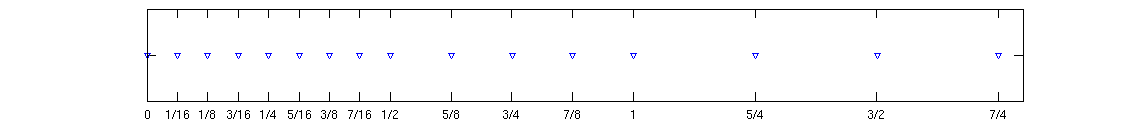
\includegraphics[width=1.0\linewidth]{figs/fp4bit}
\end{center}
\end{itemize}
\end{frame}

% -------------------------------------------------
\begin{frame}{Problems with the 5-bit Float}{Part 1}
\begin{itemize}
    \item 1. \textbf{Loss due to Normalization}:  
      If we require the leading mantissa bit to be $1$, then values like  
      $1/16,\ 1/8,\ 3/16$ cannot appear in normalized form.
\begin{center}
\pgfimage[width=1.0\linewidth]{figs/fp4bit}
\end{center}
\begin{center}
\pgfimage[width=1.0\linewidth]{figs/fp4bitnormalized}
\end{center}

    \item 2. \textbf{Overflow}:  
      Maximum value is $7/4$. Multiplying $\hat{x}=7/4$ by itself yields
      $$ \hat{x} \times \hat{x} =7/4\times 7/4 = 28/16 = ???$$

    \item 3. \textbf{Underflow}: There is no representable value between $0$ and $1/8$. Multiplying 
      $\hat{x}_1=1/8$ by $\hat{x}_2=1/2$ yields
      $$ \hat{x}_1 \times \hat{x}_2 =1/8\times 1/2 = 1/16 = ???$$
      

\end{itemize}
\end{frame}

% -------------------------------------------------
\begin{frame}{Problems with the 5-bit Float}{Part 2}
\begin{itemize}
    \item 4. \textbf{Redundancy}:  
      Different bit patterns represent the same number.  
      $$ (.100)_2 \times 2^{0} = (.010)_2 \times 2^{1} = 1/2.$$

    \item 5. \textbf{Unsigned Only}:  
      With no sign bit, the format cannot represent negative numbers.  
      Half of the real line is missing.

\end{itemize}

\bigskip
\keyidea{
Our 5-bit example reveals the essential difficulties in floating-point design.
These are exactly the issues the IEEE-754 standard solves.
}
\end{frame}

% ------------------------- -----------------------
\sectionframe{IEEE Floating Point Standard}
% -------------------------------------------------
\begin{frame}{What is the proper float representation?}
\begin{itemize}
    \item \textbf{Goal}: Find an acceptable strategy to represent $x \in (-\infty,\infty).$
    \item \textbf{Limitation}: Computers can use a finite number of bits
    \begin{center}$x\approx \hat{x}=$
    \begin{tabular}{|c|c|c||c|c| c|}\hline
      $.d_1$ & $\cdots$ & $d_m$ & $e_1$ & $\cdots$&$e_2$\\\hline
    \end{tabular}
    \end{center}
\end{itemize}

\begin{block}{Considerations}
    \begin{itemize}
        \item cover a wide range of real numbers
        \item represent positive and negative numbers 
        \item minimize the redundancy of bit sequences 
        \item lower risk of underflow 
        \item lower risk of overflow 
        \item lower risk of rounding errors
    \end{itemize}
\end{block}
\end{frame}
% -------------------------------------------------
\begin{frame}{IEEE-754}
\begin{itemize} 
\item In 19870s all computer companies \textbf{had their own representation} which lead to \textbf{different results} even with the same software

\bigskip

  \item IEEE-754 (adopted 1985) established a standard representation
    \begin{itemize}
       \item Scientists gathered to establish a memory-efficient way to represent numbers
      \item Defines the floating point distribution for our computation
      \item Offers several rounding modes which effect accuracy
    \end{itemize}
    \bigskip

    \keyidea{  
      \begin{itemize}
      \item \textbf{Unified} floating points and arithmetic across all computers
      \item Rounding errors have became more predictable and easier to study
    \end{itemize}
    }
\end{itemize}
\end{frame}
% -------------------------------------------------
\begin{frame}{IEEE Floating Point Format (IEEE-754)}
  \begin{itemize}
  \item IEEE memory is built around \textbf{words} - 32 bits of memory 

 \item IEEE may use one word, two words, or four words for representing $x\in \mathbb{R}$

\item \textbf{Single-precision} refers to using one word 
\begin{center}
  \pgfimage[width=7cm]{figs/ieee_single}
\end{center}

  \item \textbf{Double-precision} refers to using two words
\begin{center}
  \pgfimage[width=8cm]{figs/ieee_double}
\end{center}
  \item Matlab uses double precision
\end{itemize}
\end{frame}
% -------------------------------------------------
% -------------------------------------------------
\begin{frame}{IEEE Single Precision Floating Point Format}


{\define{IEE Single Precision Float (FP32)}{
The \textbf{single precision float} has the form
\begin{equation*}
  x = \pm q \times 2^m.
\end{equation*}
It occupies 32 bits of memory. It is a specific standard format set by IEEE 755.
}}
\begin{center}
  \pgfimage[width=8cm]{figs/ieee_single}
\end{center}

\begin{block}{Allocation}
\begin{itemize}
  \item 1 bit for sign $\pm $
  \item 8 bits for integer exponent is $m$
  \item 23 bits floating point mantissa $q$
  
\end{itemize}
\end{block}
\end{frame}
% -------------------------------------------------
\begin{frame}{IEE Mantissa}
\begin{center}
  \pgfimage[width=9cm]{figs/ieee_single}
\end{center}
    \begin{block}{Mantissa}
    \begin{itemize} 
        \item Entirely composed of 1s and 0s
        \item Has a \textbf{hidden bit}, always assumed to be 1 (no memory)
        \item Hidden bit reduces redundancy of the bit sequence
        \item The mantissa is computed as 
            $$ 
            q = (1.b_{22} b_{21} \ldots b_1 b_0)_{2}
            $$
        \end{itemize}
    \end{block}

\end{frame}
% -------------------------------------------------
\begin{frame}{IEE Exponent}
\begin{center}
  \pgfimage[width=9cm]{figs/ieee_single}
\end{center}

    \begin{block}{Exponent}
    \begin{itemize}   
        \item The exponent $m$ needs to be able to attain positive and negative numbers
        \item IEEE exponent is in \textbf{biased form} \\
        \item The biased form makes sure the exponent is properly ordered with respect to the bit sequence \\
        \item The exponent is computed 
        $$
            m = (b_{30} b_{29} \ldots b_{23})_2 - 127
        $$
    \end{itemize}
    \end{block}
    \begin{itemize}
        \item The exponent is in the form $m = c - o$.
        \item The $c$ is the 8-bit integer $c=(b_{30} b_{29} \ldots b_{23})_2$
        \item The integer $o$ is called the \textbf{offset} 
        \item The offset is $o = 2^{7}-1 =127$
    \end{itemize}
\end{frame}
% -------------------------------------------------
\begin{frame}{Why Biased?}
    \begin{block}{Consider the non-biased signed integer}
        $$
        m_1 =  \begin{tabular}{|c|c|c|c|c|c|c|c|}\hline
        $\pm$ & $e_0$ & $e_1$ & $e_2$ & $e_3$ & $e_4$ & $e_5$ & $e_6$ \\\hline
        \end{tabular}$$
\begin{itemize}
    \item Minimum: $ \begin{tabular}{|c|c|c|c|c|c|c|c|}\hline
        $-$ & $1$ & $1$ & $1$ & $1$ & $1$ & $1$ & $1$ \\\hline
        \end{tabular}=-127$
    \item Maximum: $ \begin{tabular}{|c|c|c|c|c|c|c|c|}\hline
        $+$ & $1$ & $1$ & $1$ & $1$ & $1$ & $1$ & $1$ \\\hline
        \end{tabular}=127$ 
    \item It has a redundant $\pm 0$\\[3mm] 
\end{itemize}
    \end{block}
\begin{block}{Consider the biased integer}
        $$
        m_2 =  \begin{tabular}{|c|c|c|c|c|c|c|c|}\hline
         $e_0$ & $e_1$ & $e_2$ & $e_3$ & $e_4$ & $e_5$ & $e_6$ & $e_7$ \\\hline
        \end{tabular} - 127$$
\begin{itemize}
    \item Minimum:  $ \begin{tabular}{|c|c|c|c|c|c|c|c|}\hline
        $0$ & $0$ & $0$ & $0$ & $0$ & $0$ & $0$ & $0$ \\\hline
        \end{tabular}=-127$
    \item Maximum: $ \begin{tabular}{|c|c|c|c|c|c|c|c|}\hline
        $1$ & $1$ & $1$ & $1$ & $1$ & $1$ & $1$ & $1$ \\\hline
        \end{tabular}=255-127 = 128$ 
    \item No redundancy
    \item Bit sequences are ordered from least to greatest
\end{itemize}
\end{block}

\end{frame}
% -------------------------------------------------
\begin{frame}{IEEE Single Precision}

\begin{example}
    Express the number $x = -52.125$ as a bit sequence in FP32.
\end{example}

\begin{enumerate}
  \item Convert base-10 to base-2 
  $$ (-52.125)_{10}=-(110100.00100000000)_2$$
  \item Convert to $1.f$ exponential form:
    $$x=\underbrace{-}_{1}(1.\underbrace{101\,000\,010\,000\,\dots\,0}_{23})_2\times
2^{5}$$
  \item Calculate exponent: $5 = c-127 \Rightarrow c = 132 \Rightarrow c =
(\underbrace{10\,000\,100}_{8})_2$
\item Write the bit sequence
\end{enumerate}

\begin{equation*}
\underbrace{1}_{1}
\underbrace{10\,000\,100}_{8}
\underbrace{101\,000\,010\,000\,\dots\,0}_{23}
\end{equation*}
\end{frame}
% -------------------------------------------------
\begin{frame}{IEEE Double Precision Floating Point Format}

{\define{IEE Double Precision Float (FP64)}{
The \textbf{double precision float} has the form
\begin{equation*}
  x = \pm q \times 2^m.
\end{equation*}
It occupies 64 bits of memory. It is a specific standard format set by IEEE 755.  
}}
\begin{center}
  \pgfimage[width=8cm]{figs/ieee_double}
\end{center}

\begin{block}{Allocation}
\begin{itemize}
  \item 1 bit for sign
  \item 11 bits for exponent
  \item 52 bits for mantissa
\end{itemize}
\end{block}
\end{frame}
% -------------------------------------------------
\begin{frame}{FP32 vs FP64: A Comparison}

\begin{center}
\begin{tabular}{|l|c|c|}
\hline
\textbf{Feature} & \textbf{FP32 (Single)} & \textbf{FP64 (Double)} \\
\hline
\textbf{Total Bits}         & 32 bits            & 64 bits \\
\textbf{Sign Bit}           & 1                  & 1 \\
\textbf{Exponent Bits}      & 8                  & 11 \\
\textbf{Mantissa Bits}      & 23                 & 52 \\
\textbf{Exponent Bias}      & 127                & 1023 \\
\textbf{Significant Digits (approx)} & 7           & 15–16 \\
\textbf{Machine Epsilon}    & $2^{-23} \approx 1.19\times10^{-7}$ & $2^{-52} \approx 2.22\times10^{-16}$ \\
\textbf{Used In}            & GPUs, mobile devices & Scientific computing \\
\hline
\end{tabular}
\end{center}

\vspace{2mm}
\keyidea{
FP64 offers much higher precision and range, at the cost of memory and performance. Matlab uses FP64.
}

\end{frame}

\begin{frame}[fragile]{Real Numbers vs. Matlab Numbers}

\define{Floating point representation}{Let $x\in\mathbb{R}$. The \textbf{floating-point representation} of $x$ is denoted $\mathrm{fl}(x)$ is the nearest representable number in the working precision. }
\begin{example}
    If $x = 0.2$, then what is $\mathrm{fl}(x)$ in Matlab? 
\end{example}
\begin{itemize}
    \begin{lstlisting}
>> fprintf('%.25f',0.2)
0.2000000000000000111022302
\end{lstlisting}
    \item On paper, $x=0.2\in\mathbb{R}$
    \item In Matlab, $\mathrm{fl}(x)=0.2000000000000000111022302\ldots$
\end{itemize}
\end{frame}

\begin{frame}{IEE-754}

\begin{figure}
    \centering
    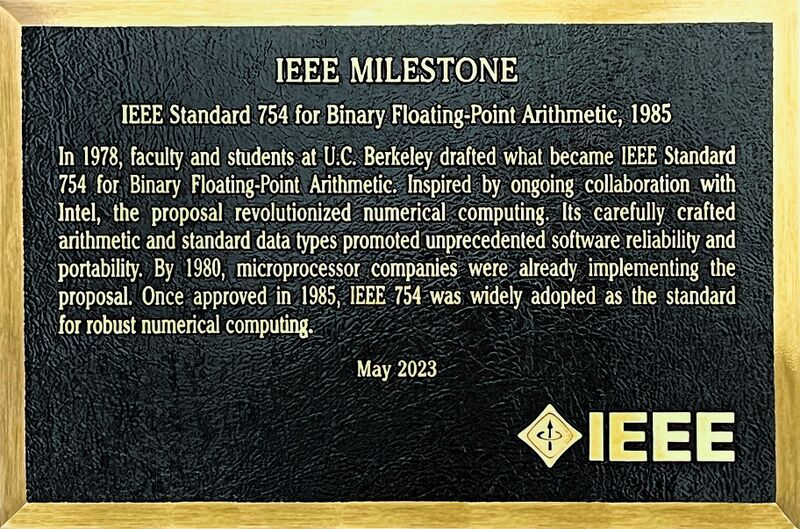
\includegraphics[width=0.75\linewidth]{figs/ieee-plaque.jpg}
\end{figure}

\keyidea{
\begin{itemize}
    \item Standardized floats was important for reproducibility 
    \item Important milestone for \textbf{numerical error analysis}
\end{itemize}
}
    
\end{frame}
% -------------------------------------------------
\sectionframe{Story}
% -------------------------------------------------
\begin{frame}[shrink]{Intel}
\begin{alertblock}{}
    Who cares about a small amount of rounding error?
\end{alertblock}
\pgfimage[width=\textwidth]{figs/intel1}
\end{frame}
% % -------------------------------------------------
% % -------------------------------------------------
\begin{frame}[shrink]{Intel}
\pgfimage[width=\textwidth]{figs/intel2}\\[5mm]
\begin{itemize}
    \item A small error was discovered in the floating point arithmetic\\[3mm]

    \item Intel's response: don't worry about it
\end{itemize}
\end{frame}
% % -------------------------------------------------
% % -------------------------------------------------
\begin{frame}[shrink]
\frametitle{Intel}
\pgfimage[width=\textwidth]{figs/intel4}
\end{frame}
% -------------------------------------------------
% -------------------------------------------------
\begin{frame}
\frametitle{Intel Timeline}
\framesubtitle{from emery.com}
\begin{description}
\item[June 1994]  Intel engineers discover the division error.  Managers
decide the error will not impact many people.  Keep the issue internal.
\item[June 1994] Dr Nicely at Lynchburg College notices computation problems
\item[Oct 19, 1994] After months of testing, Nicely confirms that other
errors are not the cause.  The problem is in the Intel Processor.
\item[Oct 24, 1994] Nicely contacts Intel.  Intel duplicates error.
\item[Oct 30, 1994] After no action from Intel, Nicely sends an email
\end{description}
\end{frame}
% -------------------------------------------------
% -------------------------------------------------
\begin{frame}[containsverbatim,shrink]
\frametitle{Intel Timeline}
\framesubtitle{from emery.com}
\begin{center}
    
\begin{block}{}
\begin{verbatim}
FROM:  Dr. Thomas R. Nicely
       Professor of Mathematics
       Lynchburg College
       1501 Lakeside Drive
       Lynchburg, Virginia 24501-3199

       Phone:     804-522-8374
       Fax:       804-522-8499
       Internet:  nicely@acavax.lynchburg.edu

TO:    Whom it may concern

RE:    Bug in the Pentium FPU

DATE:  30 October 1994

It appears that there is a bug in the floating point unit
(numeric coprocessor) of many, and perhaps all, Pentium
processors.

In short, the Pentium FPU is returning erroneous values 
for certain division operations. For example,
     0001/824633702441.0
is calculated incorrectly (all digits beyond the eighth
significant digit are in error). This can be verified in
compiled code, an ordinary spreadsheet such as Quattro Pro
or Excel, or even the Windows calculator (use the
scientific mode), by computing
     00(824633702441.0)*(1/824633702441.0),
which should equal 1 exactly (within some extremely small
rounding error; in general, coprocessor results should 
contain 16 significant decimal digits).  However, the
Pentiums tested return
     0000.999999996274709702
.
.
.
\end{verbatim}
\end{block}
\end{center}
\end{frame}
% -------------------------------------------------
% -------------------------------------------------
\begin{frame}
\frametitle{Intel Timeline}
\framesubtitle{from emery.com}
\begin{description}
\item[Nov 1, 1994]  Software company Phar Lap Software receives Nicely's
email.  Sends to colleagues at Microsoft, Borland, Watcom, etc.
decide the error will not impact many people.  Keep the issue internal.
\item[Nov 2, 1994]  Email with description goes global.
\item[Nov 15, 1994] USC reverse-engineers the chip to expose the problem.
Intel still denies a problem.  Stock falls.
\item[Nov 22, 1994] CNN \emph{Moneyline} interviews Intel.  Says the problem
is minor.
\item[Nov 23, 1994] The MathWorks develops a fix.
\item[Nov 24, 1994] New York Times story.  Intel still sending out flawed
chips.  Will replace chips only if it caused a problem in an important
application.
\item[Dec 12, 1994] IBM halts shipment of Pentium based PCs
\item[Dec 16, 1994] Intel stock falls again.
\item[Dec 19, 1994] More reports in the NYT: lawsuits, etc.
\item[Dec 20, 1994] Intel admits.  Sets aside \$420 million to fix.
\end{description}
\end{frame}

% -------------------------------------------------
\begin{frame}{Rounding Error: A Critical Concern}
\vspace{0.5cm}

\textbf{How rounding errors escalate:}
\begin{enumerate}
    \item Initial calculations introduce minor errors.
    \item Errors are compounded by multiple floating-point operations.
    \item Computer program outputs a \textbf{significantly inaccurate result}.
    \item Scientists unknowingly \textbf{rely on the flawed result}.
    \item Disaster.
\end{enumerate}

\bigskip 

\textbf{Topics to explore:}
\begin{itemize}
    \item Error propagation: Understanding how errors spread.
    \item Ill-conditioned problems: When small changes cause large effects.
\end{itemize}

\keyidea{Rounding error can lead to large errors if not handled properly. Scientists and engineers rely on numerical computations for applications.}
\end{frame}
% -------------------------------------------------
% -------------------------------------------------
\begin{frame}{Our Mission as Numerical Analysts}

\textbf{Our objectives:}
\begin{enumerate}
    \item Develop solutions that are \textit{resilient} to large roundoff errors.
    \item Achieve results with \textit{tolerable} truncation errors.
\end{enumerate}

\bigskip 

\textbf{How do we accomplish this?}
\begin{itemize}
    \item Integrate knowledge of roundoff and truncation errors into:
    \begin{itemize}
        \item Mathematical modeling
        \item Computational methods
        \item Algorithm design
        \item Software development
    \end{itemize}
    \item Promote \textit{awareness} for accurate result interpretation.
\end{itemize}
\end{frame}

% -------------------------------------------------
\begin{frame}{Yes, you have to know floats}

\begin{center}

\includegraphics[scale=0.4]{figs/meme-floats.jpg}
\end{center}
\end{frame}


\end{document}
